\documentclass[12pt,a4paper]{article}

\usepackage[T1]{fontenc}
\usepackage[polish]{babel}
\usepackage[utf8]{inputenc}
\usepackage{lmodern}
\selectlanguage{polish}
\usepackage{graphicx}
\usepackage[style=numeric,backend=biber]{biblatex}
\usepackage{csquotes}
\usepackage{float}
\usepackage{amsmath}


\addbibresource{bib.bib} 

\begin{document}

\nocite{*}

\pagenumbering{gobble}
\clearpage

\begin{figure}[h]
\centering

\includegraphics[width=0.4\textwidth]{media/ps-logo.png} 
\end{figure}

\hspace{3cm}
\begin{center}Dokumentacja projektowa\end{center}
\begin{center}MLA 2025/2026\end{center}
\hspace{3cm}

\begin{center}
\large\textbf{Aplikacje uczenia maszynowego \\w systemach interakcji człowiek-maszyna}
\end{center}

\hspace{7cm}
\begin{flushright}
Kierunek: Informatyka \\ 
Specjalność: Uczenie Maszynowe \\
Stopień: II
\end{flushright}

\begin{flushright}
Członkowie zespołu:
\par
\textit{Piotr Skowroński - Lider Zespołu i Specjalista LaTeX}
\par
\textit{Krzysztof Czuba - Inżynier ML}
\par
\textit{Kinga Grabarczyk - Inżynier Danych}
\par
\textit{Irek Kosek - Specjalista HCI}
\end{flushright}

\vfill
\begin{center}Gliwice, 2025/2026\end{center}

\newpage

\pagenumbering{arabic}
\tableofcontents

\newpage

\section{Wprowadzenie}
Niniejsza dokumentacja opisuje projekt zespołowy realizowany w ramach przedmiotu "Aplikacje uczenia maszynowego w systemach interakcji człowiek-maszyna". Projekt skupia się na problemie segmentacji obrazów medycznych w celu wykrywania zmian nowotworowych płuc.

\subsection{Cel projektu}
Głównym celem jest opracowanie i wytrenowanie modelu głębokiego uczenia, który pozwoli na automatyczne wyodrębnienie obszarów zajętych chorobą ze skanów tomografii komputerowej (CT). System ma służyć jako interaktywne wsparcie dla radiologa, przyspieszając proces diagnostyczny.

\subsection{Zespół projektowy}
Imię i Nazwisko 1 :: Inżynier ML :: Implementacja modelu MONAI UNet, pętla treningowa, ewaluacja metryk. \\
Imię i Nazwisko 2 :: Specjalista HCI :: Projektowanie interfejsu interakcji, analiza Mapy Myśli, dokumentacja.

\newpage

\section{Założenia projektowe}
Projekt realizowany jest zgodnie z metodyką Project-based learning, uwzględniając analizę źródeł naukowych dotyczących głębokich sieci splotowych w medycynie.

\subsection{Koncepcja i Mapa Myśli}
Proces konceptualizacji projektu został utrwalony w formie mapy myśli, uwzględniającej aspekty techniczne (ML) oraz użytkowe (HCI).

\begin{figure}[h]
\centering
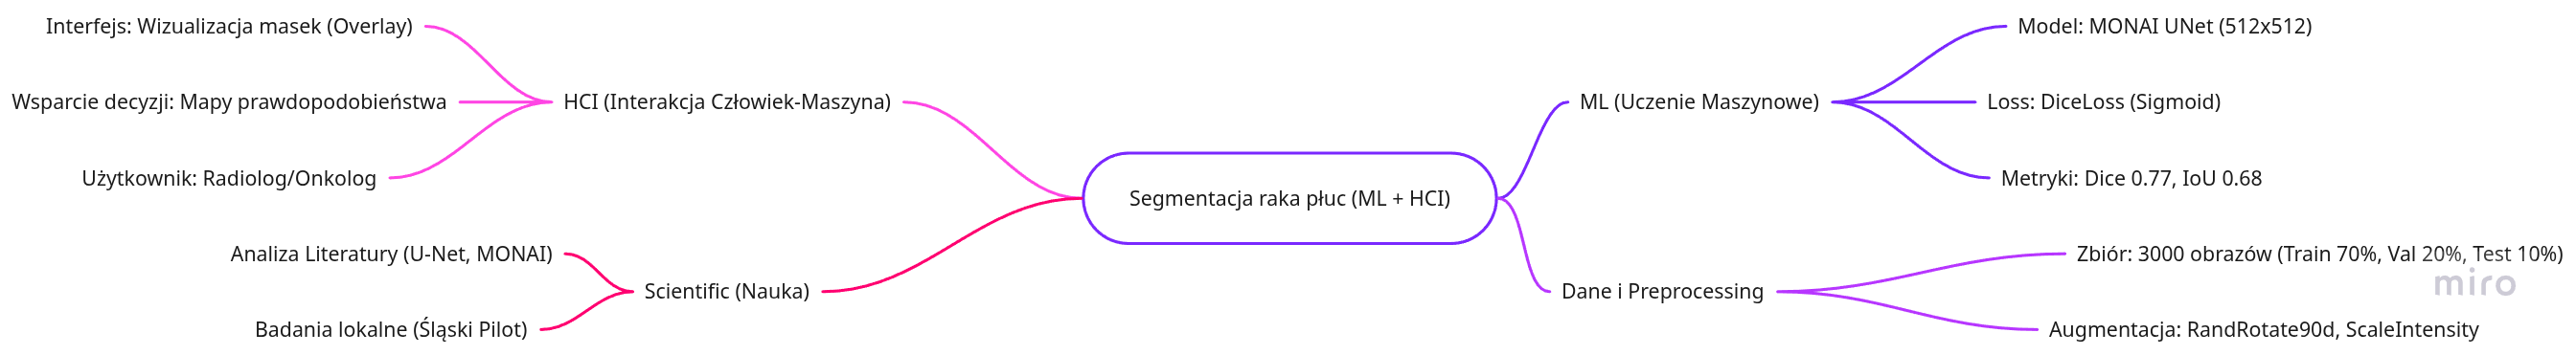
\includegraphics[width=\textwidth,height=0.15\textheight]{media/mind_map.png}
\caption{Mapa myśli procesu konceptualizacji projektu.}
\end{figure}

\subsection{Zbiór danych i transformacje}
W projekcie wykorzystano publicznie dostępny zbiór danych \textbf{Lung Cancer Segmentation Dataset} pochodzący z platformy Kaggle. Dataset składa się z 3000 par obrazów: skanów tomografii komputerowej (CT) płuc oraz odpowiadających im masek segmentacyjnych przygotowanych przez ekspertów radiologów.

\subsubsection{Charakterystyka zbioru danych}
\begin{itemize}
    \item \textbf{Źródło:} Kaggle - Lung Cancer Segmentation Dataset.
    \item \textbf{Liczba próbek:} 3000 par (obraz CT + maska ekspercka).
    \item \textbf{Format obrazów:} Pliki graficzne w skali szarości.
    \item \textbf{Typ adnotacji:} Binarne maski segmentacyjne oznaczające obszary zmian nowotworowych.
    \item \textbf{Podział danych:} 70\% trening, 20\% walidacja, 10\% test.
\end{itemize}

\subsubsection{Transformacje i augmentacja}
Zastosowano następujące transformacje danych w celu przygotowania ich do procesu uczenia:
\begin{itemize}
    \item \textbf{Normalizacja intensywności:} Skalowanie wartości pikseli do zakresu [0, 1] w celu stabilizacji procesu uczenia.
    \item \textbf{Augmentacja geometryczna:} Losowa rotacja o wielokrotność 90 stopni (prawdopodobieństwo p=0.5) w celu zwiększenia różnorodności danych treningowych i redukcji przeuczenia.
    \item \textbf{Konwersja typów:} Transformacja do tensorów PyTorch typu float32.
\end{itemize}

\newpage

\section{Implementacja}

\subsection{Architektura modelu}
W projekcie wykorzystano architekturę \textbf{U-Net}, która została zaproponowana przez Ronnebergera i współpracowników w 2015 roku specjalnie do zadań segmentacji obrazów biomedycznych.

\subsubsection{Opis architektury U-Net}
Architektura U-Net charakteryzuje się symetryczną strukturą w kształcie litery „U", składającą się z dwóch głównych części:

\begin{itemize}
    \item \textbf{Ścieżka kurczenia (Encoder/Contracting Path):} Lewa strona sieci odpowiedzialna za ekstrakcję cech. Składa się z powtarzających się bloków: dwóch warstw konwolucyjnych 3x3 z aktywacją ReLU, po których następuje warstwa max pooling 2x2. Na każdym poziomie liczba kanałów cech jest podwajana, co pozwala na wychwytywanie coraz bardziej abstrakcyjnych reprezentacji obrazu.

    \item \textbf{Ścieżka ekspansji (Decoder/Expanding Path):} Prawa strona sieci odpowiedzialna za rekonstrukcję przestrzenną. Wykorzystuje warstwy up-convolution (transpozycja konwolucyjna) 2x2 w celu zwiększenia rozdzielczości, połączone z odpowiadającymi mapami cech ze ścieżki kurczenia poprzez mechanizm \textit{skip connections}.

    \item \textbf{Skip Connections:} Kluczowy element architektury, który łączy odpowiadające poziomy enkodera i dekodera. Umożliwia to zachowanie szczegółowych informacji przestrzennych, które są tracone podczas operacji pooling, co jest szczególnie istotne dla precyzyjnej lokalizacji granic segmentowanych obiektów.
\end{itemize}

\subsubsection{Konfiguracja modelu w MONAI}
Wykorzystano implementację UNet z biblioteki MONAI (Medical Open Network for AI) o następujących parametrach:
\begin{itemize}
    \item \textbf{Wymiary przestrzenne:} 2D (spatial\_dims=2).
    \item \textbf{Kanały wejściowe:} 1 (obrazy w skali szarości).
    \item \textbf{Kanały wyjściowe:} 1 (binarna maska segmentacyjna).
    \item \textbf{Struktura kanałów:} (16, 32, 64, 128, 256) — liczba filtrów na kolejnych poziomach.
    \item \textbf{Strides:} (2, 2, 2, 2) — krok redukcji przestrzennej między poziomami.
\end{itemize}

\subsection{Proces treningowy}

\subsubsection{Funkcja straty — Dice Loss}
W zadaniach segmentacji obrazów medycznych często występuje problem niezrównoważenia klas — obszary zmian chorobowych zajmują znacznie mniejszą część obrazu niż tło. Klasyczna funkcja straty cross-entropy w takich przypadkach może prowadzić do słabych wyników. Z tego powodu zastosowano funkcję straty \textbf{Dice Loss}.

Dice Loss jest bezpośrednio powiązana ze współczynnikiem Dice (Dice Coefficient) i definiowana jest jako:

\begin{equation}
\text{Dice Loss} = 1 - \frac{2 \sum_{i=1}^{N} p_i \cdot g_i + \epsilon}{\sum_{i=1}^{N} p_i + \sum_{i=1}^{N} g_i + \epsilon}
\end{equation}

gdzie:
\begin{itemize}
    \item $p_i$ — wartość predykcji dla piksela $i$ (po aktywacji sigmoid),
    \item $g_i$ — wartość ground truth dla piksela $i$ (0 lub 1),
    \item $N$ — całkowita liczba pikseli,
    \item $\epsilon$ — mały współczynnik wygładzający (smooth factor) zapobiegający dzieleniu przez zero.
\end{itemize}

\textbf{Zalety Dice Loss:}
\begin{itemize}
    \item Naturalna odporność na niezrównoważenie klas.
    \item Bezpośrednia optymalizacja metryki używanej do ewaluacji.
    \item Lepsza konwergencja dla obiektów o małej powierzchni.
\end{itemize}

\subsubsection{Konfiguracja procesu uczenia}
Model trenowano z użyciem następujących parametrów:
\begin{itemize}
    \item \textbf{Optymalizator:} Adam z początkowym tempem uczenia $lr=0.001$.
    \item \textbf{Funkcja straty:} DiceLoss z aktywacją sigmoid.
    \item \textbf{Scheduler:} ReduceLROnPlateau — dynamiczna redukcja tempa uczenia o czynnik 0.1 przy braku poprawy przez 10 epok.
    \item \textbf{Liczba epok:} 400.
    \item \textbf{Rozmiar batcha:} 64.
    \item \textbf{Early stopping:} Monitorowanie validation loss z cierpliwością 30 epok.
\end{itemize}

\newpage

\section{Badania}
Ewaluacja modelu została przeprowadzona na wydzielonym zbiorze testowym (10\% danych).

\subsection{Metryki ilościowe}

\subsubsection{Dice Coefficient (Współczynnik Dice / F1-Score)}
Współczynnik Dice, znany również jako Sørensen-Dice coefficient lub F1-Score dla segmentacji, jest jedną z najczęściej stosowanych metryk do oceny jakości segmentacji obrazów medycznych. Mierzy on podobieństwo między predykcją modelu a ground truth.

Współczynnik Dice definiowany jest jako:

\begin{equation}
\text{Dice} = \frac{2 \cdot |P \cap G|}{|P| + |G|} = \frac{2 \cdot TP}{2 \cdot TP + FP + FN}
\end{equation}

gdzie:
\begin{itemize}
    \item $P$ — zbiór pikseli zaklasyfikowanych jako pozytywne (predykcja),
    \item $G$ — zbiór pikseli ground truth (maska ekspercka),
    \item $TP$ — true positives (poprawnie wykryte piksele zmiany),
    \item $FP$ — false positives (błędnie wykryte piksele jako zmiana),
    \item $FN$ — false negatives (pominięte piksele zmiany).
\end{itemize}

Wartość Dice mieści się w przedziale [0, 1], gdzie 1 oznacza idealne dopasowanie.

\subsubsection{Intersection over Union (IoU / Jaccard Index)}
IoU (Intersection over Union), znany również jako indeks Jaccarda, jest kolejną fundamentalną metryką w segmentacji obrazów. Mierzy stosunek części wspólnej do sumy zbiorów predykcji i ground truth.

IoU definiowany jest jako:

\begin{equation}
\text{IoU} = \frac{|P \cap G|}{|P \cup G|} = \frac{TP}{TP + FP + FN}
\end{equation}

\textbf{Relacja między Dice a IoU:}
Obie metryki są ze sobą powiązane matematycznie:
\begin{equation}
\text{Dice} = \frac{2 \cdot \text{IoU}}{1 + \text{IoU}} \quad \Leftrightarrow \quad \text{IoU} = \frac{\text{Dice}}{2 - \text{Dice}}
\end{equation}

Dice zawsze przyjmuje wartości wyższe lub równe IoU dla tego samego przypadku, ponieważ bardziej premiuje część wspólną.

\subsubsection{Wyniki eksperymentalne}
Wyniki uzyskane na zbiorze testowym (300 obrazów, 10\% całego zbioru) prezentują się następująco:
\begin{itemize}
    \item \textbf{Average Dice Coefficient: 0.77} — dobry poziom zgodności segmentacji.
    \item \textbf{Average Intersection over Union (IoU): 0.68} — solidne pokrycie obszarów zmian.
    \item \textbf{Average Recall: 0.80} — wysoka czułość wykrywania zmian nowotworowych.
    \item \textbf{Average Precision: 0.78} — dobra precyzja z niskim poziomem fałszywych alarmów.
\end{itemize}

\textbf{Interpretacja wyników:}
Uzyskany współczynnik Dice na poziomie 0.77 wskazuje, że model poprawnie identyfikuje około 77\% obszaru zmiany nowotworowej przy jednoczesnym zachowaniu niskiego poziomu fałszywie pozytywnych predykcji. Wysoki Recall (0.80) jest szczególnie istotny w kontekście diagnostyki medycznej, gdzie pominięcie zmiany nowotworowej może mieć poważne konsekwencje kliniczne.

\subsection{Analiza wizualna}
Poniżej przedstawiono przebieg funkcji straty oraz przykładowe predykcje modelu na tle masek wzorcowych.

\begin{figure}[H]
\centering
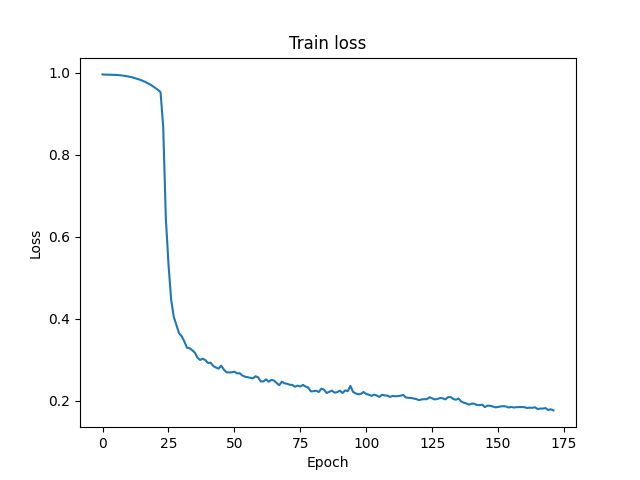
\includegraphics[width=0.8\textwidth,height=\textheight,keepaspectratio]{media/train_loss.png}
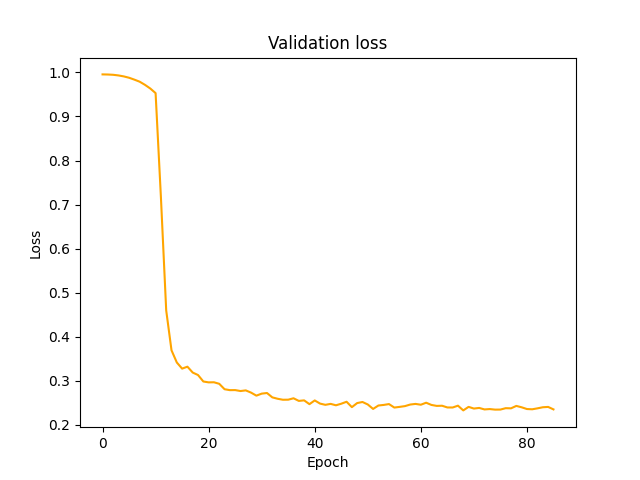
\includegraphics[width=0.8\textwidth,height=\textheight,keepaspectratio]{media/val_loss.png}
\caption{Wykresy funkcji straty dla zbioru treningowego i walidacyjnego.}
\end{figure}

\begin{figure}[H]
\centering
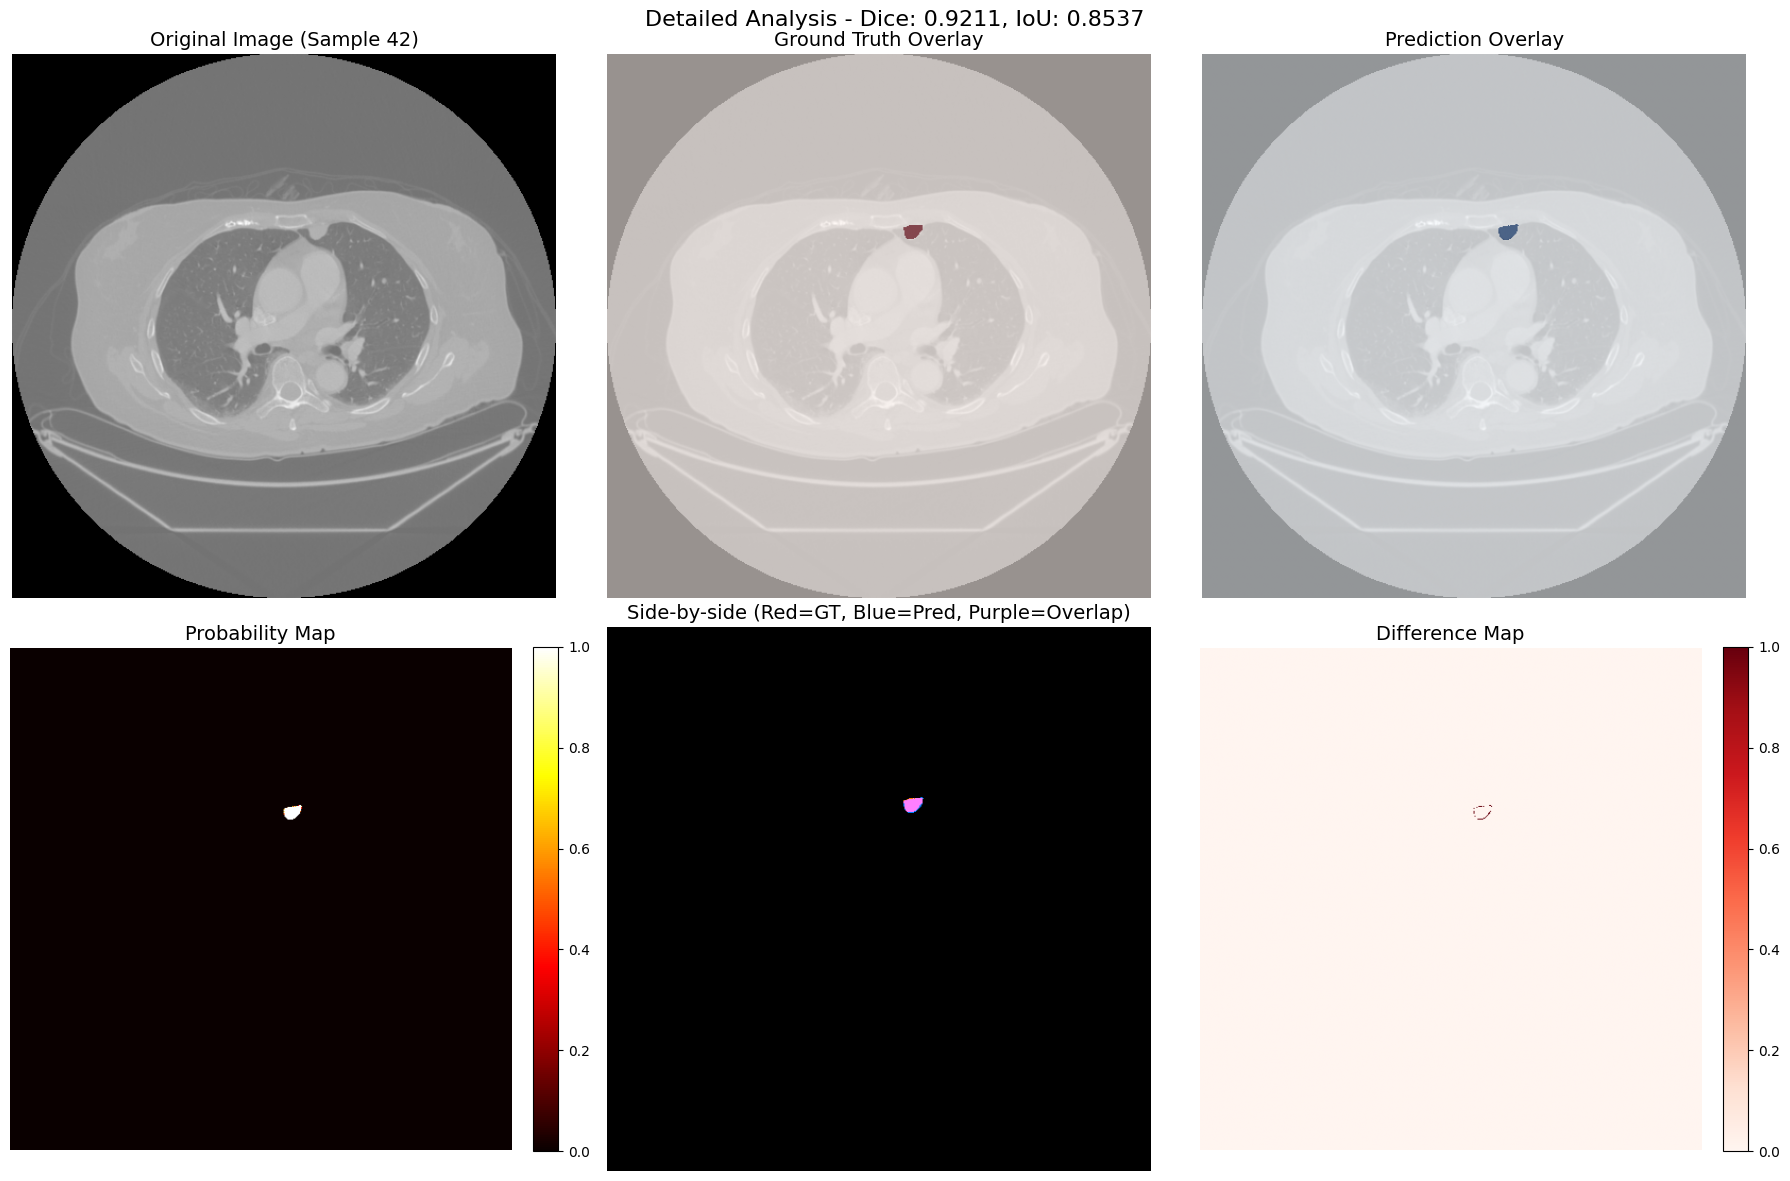
\includegraphics[width=1\textwidth,height=\textheight,keepaspectratio]{media/model_predictions_comparison.png}
\caption{Wizualizacja predykcji: Obraz oryginalny, Ground Truth, Predykcja oraz Nałożenie.}
\end{figure}

\newpage

\section{Podsumowanie i wnioski}

\begin{itemize}
    \item \textbf{Podsumowanie:} W ramach projektu pomyślnie wytrenowano model UNet z biblioteki MONAI na zbiorze 3000 obrazów CT. Model osiągnął satysfakcjonujące wyniki metryczne: współczynnik Dice na poziomie 0,77 oraz IoU równy 0,68. Proces treningu (400 epok) przebiegał stabilnie, co potwierdzają wygenerowane wykresy funkcji straty, wykazujące zbieżność zarówno na zbiorze treningowym, jak i walidacyjnym.
    \item \textbf{Wnioski techniczne (ML):} Wysoka wartość metryki Recall (0,80) w stosunku do Precision (0,78) sugeruje, że model jest dobrze zoptymalizowany pod kątem czułości diagnostycznej. W badaniach przesiewowych raka płuc priorytetem jest minimalizacja wyników fałszywie ujemnych, co udało się osiągnąć. Analiza map różnicowych (Difference Maps) wskazuje, że ewentualne błędy wynikają głównie z trudności w precyzyjnym wyznaczaniu granic mniejszych zmian nowotworowych.
    \item \textbf{Wnioski HCI:} Zastosowanie nakładek wizualnych (Overlay Comparison) oraz map prawdopodobieństwa stanowi kluczowy element interakcji człowiek-maszyna. Pozwala to radiologowi na błyskawiczną weryfikację obszarów wskazanych przez algorytm, co w praktyce klinicznej może skrócić czas opisu badania przy jednoczesnym zachowaniu wysokiej czujności diagnostycznej.
\end{itemize}


\newpage
\section{Spis literatury}
\printbibliography[heading=none] 

\end{document}